\section{From Na\"{i}ve Bayes to Deep Neural Networks}
\label{sec:nb2dnn}
To do supervised machine learning, we can use several models, all of which have
different advantages and disadvantages, and are more useful for some use cases
than for others.

We will discuss the most common ones in this chapter.

\todo[inline]{add all code examples}


\subsection{Na\"ive Bayes}
The Na\"ive Bayes classifier is a very simple classifier that is often used as
a ``baseline''. Before estimating more complicated and resource-intensive models,
it is a good idea to estimate a simpler model first, to assess how much better the
other model actually is. Sometimes, the simple model might even be just fine.

The Na\"ive Bayes classifier allows you to predict a binary outcome, such as:
``Is this message spam or not?'', ``Is this article about politics or not?'',
``Will this go viral or not?''.
It, in fact, also allows you to do the same with more than one category, and both
the Python and the R implementation will happily let you train a Na\"ive Bayes
classifier on nominal data, such as whether an article is about politcs, sports, the
economy, or something different.

For the sake of simplicity, we will discuss a binary example, though.

As its name suggests, a Na\"ive Bayes classifier is based on Bayes' theorem, and it is
``na\"ive''.
It may sound a bit weird to call a model ``na\"ive'', but what it actually means is
not so much that it is stupid, but that it makes very far-reaching assumptions
about the data (hence, it is na\"ive). Specifically, it assumes that all features
are independent from each other.
Of course, that is hardly ever the case -- for instance, in a survey data set,
while age and gender indeed are fully independent from each other (unless, for instance,
a war swept away a whole generation of males but not females), this is not the case
for education, political interest, media use, and so on.
And in textual data, whether a word X is used is not independent from the use of word
Y --- after all, both are not randomly drawn from a dictionary, but depend on the
topic of the text (and other things).
Astonishingly, even though these assumptions are regularly violated, the Na\"ive Bayes classifier works reasonably well in practice.

The Bayes part of the Na\"ive Bayes classifier comes from the fact that it uses Bayes formula, $$ P(A \mid B) = \frac{P(B \mid A) \, P(A)}{P(B)} $$.

As a short refresher: The $P(A \mid B)$ can be read as: the probability of A, given B. Or: the probability of A if B is the case/present/true.
Applied to our problem, this means that we are interested in estimating the probability of an item having a label, given a set of features:
$$ P(label \mid features) = \frac{P(features \mid label) \, P(label)}{P(features)} $$.

$P(label)$ can be easily calculated: It's just the fraction of all cases with the label we are interested in.
Because we assume that our features are independent (remember, the ``na\"ive'' part), we can calculate $P(features)$ and $P(features\mid label)$ by just multiplying the probabilities of each individual feature.
Let's assume we have three features, $x_1, x_2, x_3$.
We now simply calculate the percentage  of \emph{all} cases that contain these features, $P(x_1), P(x_2)$ and $P(x_3)$.
Then we do the same for the conditional probabilities and calculate  the percentage  of  cases \emph{with our label} that contain these features, $P(x_1\mid label), P(x_2\mid label)$ and $P(x_3\mid label)$.

If we fill this in our formula, we get:


$$ P(label \mid features) = \frac{P(x_1 \mid label) \cdot P(x_2 \mid label)\ \cdot P(x_3 \mid label) \cdot P(label)}{P(x_1) \cdot P(x_2) \cdot P(x_3)}$$.

Remember that all we need to do to calculate this formula is: (1) counting how many cases we have in total; (2) counting how many cases have our label; (3) counting how many cases out of [1] have feature x; (4) counting how many cases out of [2] have feature x.
As you can imagine, doing this does not take much time to do, which makes the Na\"ive Bayes classifier such a fast and efficient choice.
This may in particular be true if you have very many features (i.e., high-dimensional
data).

Counting whether a feature is present or not, of course, is only possible for binary data. We could for example simply check whether a given word is present in a text or not.
But what if our features are continous data, such as the number of times the word is present?
We could dichotomize it, but that would throw away information.
So, what we do instead, is that we estimate $P(x_i)$ using a distribution, for example
a Gaussian, Bernoulli, or multinomial distribution. The core idea, though, stays the same.



\subsection{Regression}
Regression analysis does not make as strong an assumption about the independence of features as the Na\"ive Bayes classifier does.
Sure, we have been warned about the dangers of multicollinearity in statistics classes,
but correlation between features (for which is multicollinearity is a fancy term)
affects the coefficients and their $p$ values, but not the predictions of the model
as a whole.
To put it differently, in regression models, we do not estimate the probability of a label given a feature, independent of all the other features, but are able to ``control for'' their influence.
In theory, this should make our models better, and also in practice, this regularly is
the case. However, ultimately, it is an empirical question whether this is the case.

While we started this chapter with an example of an OLS regression to estimate a
continous outcome (well, by approximation, as for ``days per week'' not all values make sense), we will now use a regression approach to predict nominal outcomes, just as in the Na\"ive Bayes example.
The type of regression analysis to use for this is called \emph{logistic regression}.

In a normal OLS regression, we estimate

$$y = \beta_o + \beta_1 x_1 + \beta_2 x_2 = \ldots + \beta_n x_n$$

But this gives us a continous outcome, which we do not want. In a logistic regression, we therefore use the sigmoid function to map this continous outcome to a value between 0 and 1. The sigmoid function is defined as
$sigmoid(z) = \frac{1}{1 + e^{-z}}$
and depicted in Figure~\ref{fig:sigmoid}.

\begin{figure}
  \centering
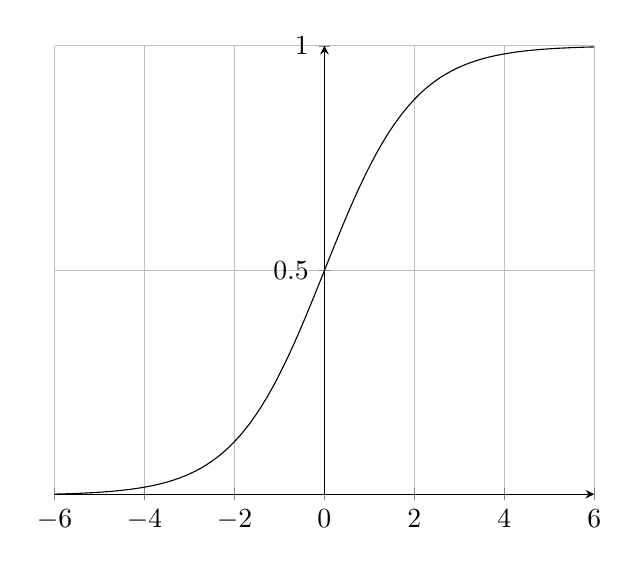
\begin{tikzpicture}
    \begin{axis}%
    [
        grid=major,     
        xmin=-6,
        xmax=6,
        axis x line=bottom,
        ytick={0,.5,1},
        ymax=1,
        axis y line=middle,
    ]
        \addplot%
        [
            black,%
            mark=none,
            samples=100,
            domain=-6:6,
        ]
        (x,{1/(1+exp(-x))});
    \end{axis}
\end{tikzpicture}
\caption{\label{fig:sigmoid} The sigmoid function}
\end{figure}


Combining these formulas gives us:

$$P = \frac{1}{1 + e^{-(\beta_o + \beta_1 x_1 + \beta_2 x_2 = \ldots + \beta_n x_n)}} $$


Wait, you might say. Isn't $P$ still continous, even though it is now bounded between 0 and 1? Yes, it is.
Therefore, after having estimated the model, we use a threshold value (typically, 0.5)
to predict the label. If $P>0.5$, we predict that the case is spam/about politics/will go viral, if not, we predict its not.

A nice side effect of this is that we still can use the probabilities in case we are interested in them, for example to figure out for which cases we are more sure in our prediction.

Just as with the Na\"ive Bayes classifier, also for logistic regression classifiers, Python and R will happily allow us to estimate models with multiple nominal outcomes instead of a binary outcome.

And, of course, you actually can do OLS regression (or more advanced regression models) if you want to estimate a continous outcome.


\subsection{Support Vector Machines}
\todo[inline]{maybe more detail/math/plots needed}
Support Vector Machines are another very popular and versatile approach to supervised machine learning.
In fact, they are quite similar to logistic regression, but try to optimize a different function. In technical terms, SVM minimizes \emph{hinge loss} instead of logistic loss.

What does that mean to us? When estimating logistic regressions, we are interested
in estimating probabilities, while when training a support vector machine, we are interested in finding a plane (more specifically, a hyperplane) that best separates the datapoints of the two classes (e.g., spam vs non-spam messages) that we want to distinguish.
This also means that a SVM does not give you probabilities associated with your prediction, but just the label.
But usually, that's all that you want anyway.

Without going into mathematical detail here (for that, a good source would be [ADD LITERATURE REFERENCE], we can say that finding the widest separating margin that we can achieve constructing a plane in a geographical space (SVM) versus optimizing a log-likelihood function (logistic regression) results in a model that is less sensitive to outliers, and tends to be more balanced.

Another advantage of SVMs is that they can be extended to non-linear separable classes. Using a so-called kernel function, we can transform our data so that the dataset becomes linearly separable. Choices include but are not limited to multinomial kernels, the radial basis function (RBF),  or Gaussian kernels. 
\todo[inline]{decide how far we want to go here}.




\subsection{Decision Trees and Random Forests}
In the models we discussed so far, we essentially were modeling linear relationships. If the value of a feature is twice as high, its influence on the outcome will be twice as high as well.
Sure, we can (and do, as in the case of the sigmoid function) apply some transformations, but we have not really considered yet how we can model situations in which, for instance, we care about whether the value of a feature is above (or below) a speciifc threshold.
For instance, if we have a set of social media messages and want to model the medium where they most likely come from, then its length is  very important information. If it is longer than 280 characters (or, historically, 14), then we can be \emph{very} sure it is not from Twitter, even though the reverse is not necessarily true. But it does not matter at all whether it is 290 or $10000$ characters long.

Entering this variable into a logistic regression, thus, would not be a smart idea.
We could, of course, dichotomize it, but that would only partly solve the problem.
More generally, in this example, we \emph{know} how to dichotomize it based on our prior knowledge about the number of characters in a tweet.

This is were decision trees come into play. Figure~\ref{fig:decisiontree} depicts a (hypothetical) decision tree.

\begin{figure}
  \centering
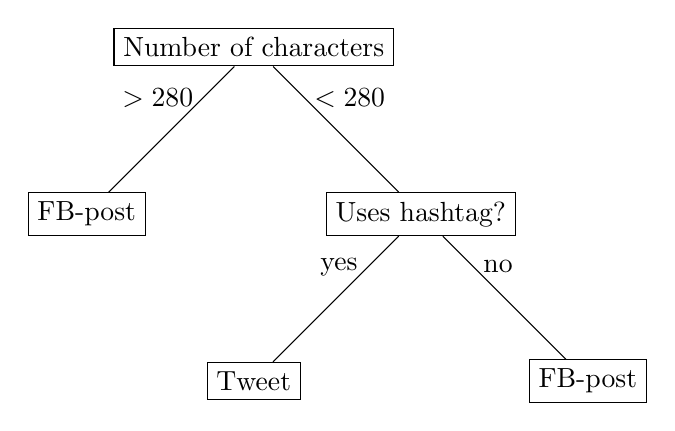
\begin{tikzpicture}[
    node/.style={%
      draw,
      rectangle,
    },
  ]

    \node [node] (A) {Number of characters};
    \path (A) ++(-135:30mm) node [node] (B) {FB-post};
    \path (A) ++(-45:30mm) node [node] (C) {Uses hashtag?};
    \path (C) ++(-135:30mm) node [node] (D) {Tweet};
    \path (C) ++(-45:30mm) node [node] (E) {FB-post};

    \draw (A) -- (B) node [left,pos=0.25] {$>280$}(A);
    \draw (A) -- (C) node [right,pos=0.25] {$<280$}(A);
    \draw (C) -- (D) node [left,pos=0.25] {yes}(A);
    \draw (C) -- (E) node [right,pos=0.25] {no}(A);
\end{tikzpicture}
  \caption{\label{fig:decisiontree}A simple decision tree}
\end{figure}

Faced with the challenge to predict whether a social media message is a tweet
or a Facebook post, we could predict 'Facebook post' if its length is greater than 280 characters. If not, we check whether it includes hashtags, and if so, we predict 'tweet', otherwise, 'Facebook post'.

Of course, this simplisitic model will be wrong at some times, because not all tweets have hashtags, and some Facebook posts actually do include hashtags.

While we construted this hypothetical decision tree by hand, usually, we are more nterested in learning such non-linear relationships from the data.
This means that we we do not have to determine the cutoff point ourselves, but also that we do not determine the order in which we check multiple variables by hand.

\todo[inline]{add stuff on how decision trees are estimated}

Decision trees have two nice properties. First, they are very easy to explain.
In fact, a figure like Figure~\ref{fig:decisiontree} is understandable for non-experts, which can be important in scenarios where for accountability reasons, the decision of a classifier must be as transparent as possible.
Second, they allow us to model non-linear relationships even if we have very little ideas about how these relationships look like.

However, this comes at large costs.
Formulating a model as a series of yes/no questions, as you can imagine, inherently uses a lot of nuance. More importantly, in such a tree, you cannot ``move up'' again. In other words, if you make a wronng decision early on in the tree (i.e., close to its root node), you cannot correct it any more.
This rigidity makes decision trees also prone to overfitting: they may fit the training data very well, but may not generalize well enough to slightly different (test) data.

Because of these drawbacks, decision trees are seldom used in real-life classification tasks.
Instead, one uses so-called random forests.
Drawing random samples from the data, we estimate multiple decision trees -- hence, a forest.
To arrive at a final prediction, we then can let the trees ``vote'' on which label we should predict. This procedure is called ``majority voting'', but there are also other methods available. For example, scikit-learn by default uses a method called probabilistic prediction, which takes into account probability values instead of simple votes.


Because random forests alleviate the problems of decision trees, but keep the advantage of being able to model non-linear relationships, they are frequently used when we expect such relationships.
Also, random forests may be a good choice if you have very different types of features (some nominal, some continous, etc.) in your model. The same holds true if you have a lot (really a lot) features: Methods like SVM would require constructing large matrices in memory, which random forests do not.
But if the relationships between your features and your labels are acually (approximately) linear, then you are probably better off with one of the other models we discussed.


\subsection{A glimpse into Deep Learning} 

An extensive treatment of Deep Learning is out of the scope of this book (we recommend XXXXX instead), but we will give you a brief introduction, so that you can decide whether it is worth diving deeper into it.

bla
bla
bla
bla
bla
